\section{Deep Learning}
\begin{itemize}
	\item Deep Neural Networks perform hierarchical feature learning and classification in a single architecture
\end{itemize}
\subsection{Convolutional Neural Networks}
\begin{itemize}
	\item Key layer of CNNs are convolutions. The weights are surface-wise local, but depth-wise global.
	\item Multiple neurons look at the same position, but using different kernels (channels)
	\item Parameters of a convolutional layer
	\begin{itemize}
		\item \textit{Kernel size}: size of the filter which is learned. If size is $k\times k$, we learn overall $k^2$ parameters per channel
		\item \textit{Input channels}: number of input channels $c_i$. Every filter has the size of $k\times k\times c_i$
		\item \textit{Output channels}: number of output channels $c_o$. Represent the number of different filters learned.
		\item \textit{Stride} with which we slide the filter over the image. Stride of $s=1$ means we apply a filter on every pixel as usual, $s=2$ would skip every second pixel and $s=4$ takes only every fourth pixel as center of an filter application. Default: $s=1$.
	\end{itemize}
	\item Overall, we learn $(k\times k\times c_i + 1)\times c_0$ \textbf{parameters} in a convolutional layer (the 1 extra parameter for bias)
	\item The \textbf{output size} is calculated by $$h_o = (h_i + 2\cdot p - k) / s + 1$$ where $p$ is the padding (number of extra pixels on each side)
	\begin{figure}[ht!]
		\centering
		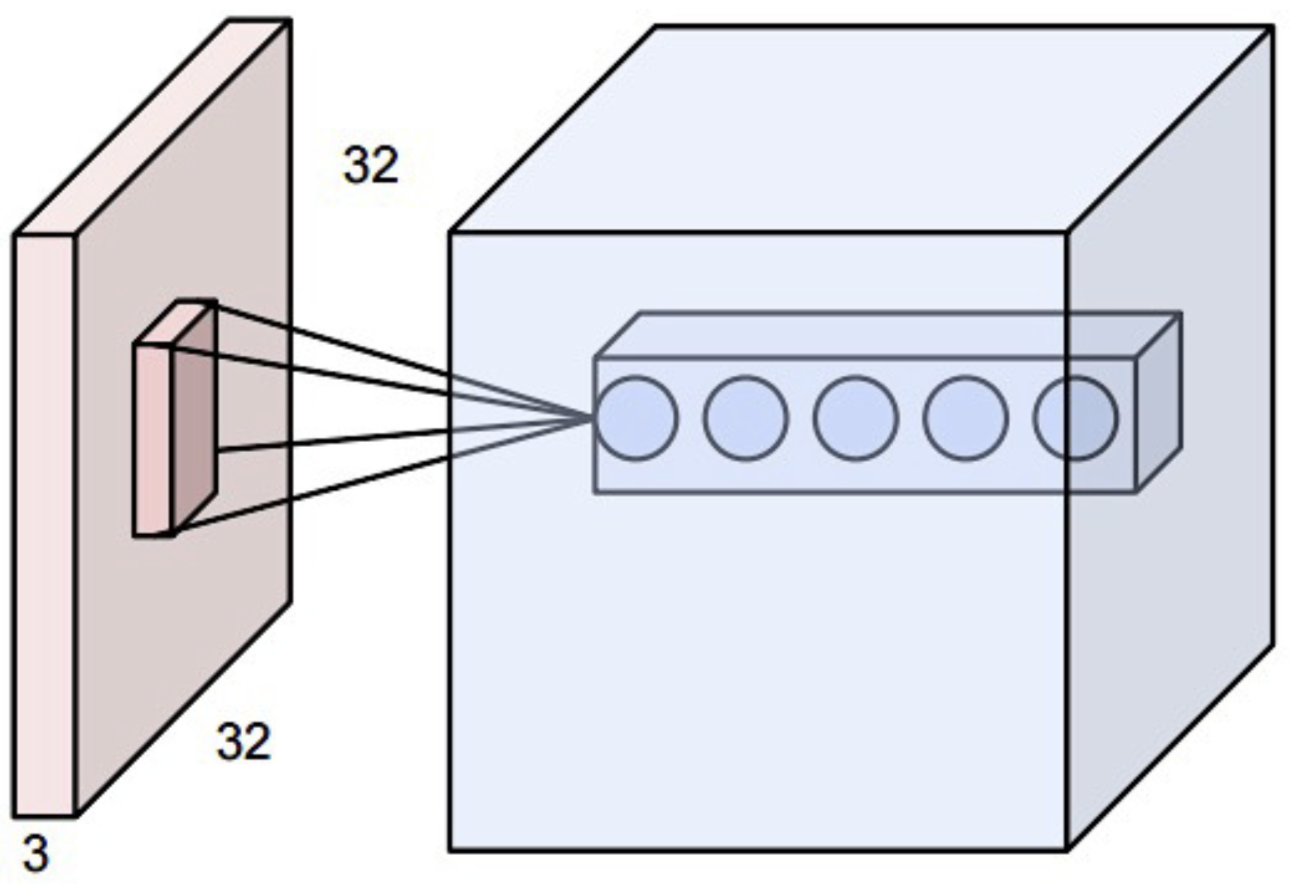
\includegraphics[width=0.2\textwidth]{figures/cv_deep_learning_convolution_operator.png}
		\caption{Convolutional layer in a CNN}
	\end{figure}
	\item Activation layers like ReLU ($\max(0,x)$) introduce non-linearity
	\item Pooling aggregates multiple values into a single value making it invariant to small transformations. Reduces the size of the next output layer while keeping the most important information 
\end{itemize}
\subsubsection{Transfer Learning}
\begin{itemize}
	\item Reuse information gained on a large dataset (e.g. ImageNet) on a new one
	\item Depending on the amount and similarity of data with the pretrained one, we should fine-tune different layers (see Figure~\ref{fig:transfer_learning})
	\item Transfer Learning can greatly influence the performance of a network. Low level features (first layers) are almost always the same for images as we have to detect edges, colors, etc.
\end{itemize}
\begin{figure}[ht!]
	\centering
	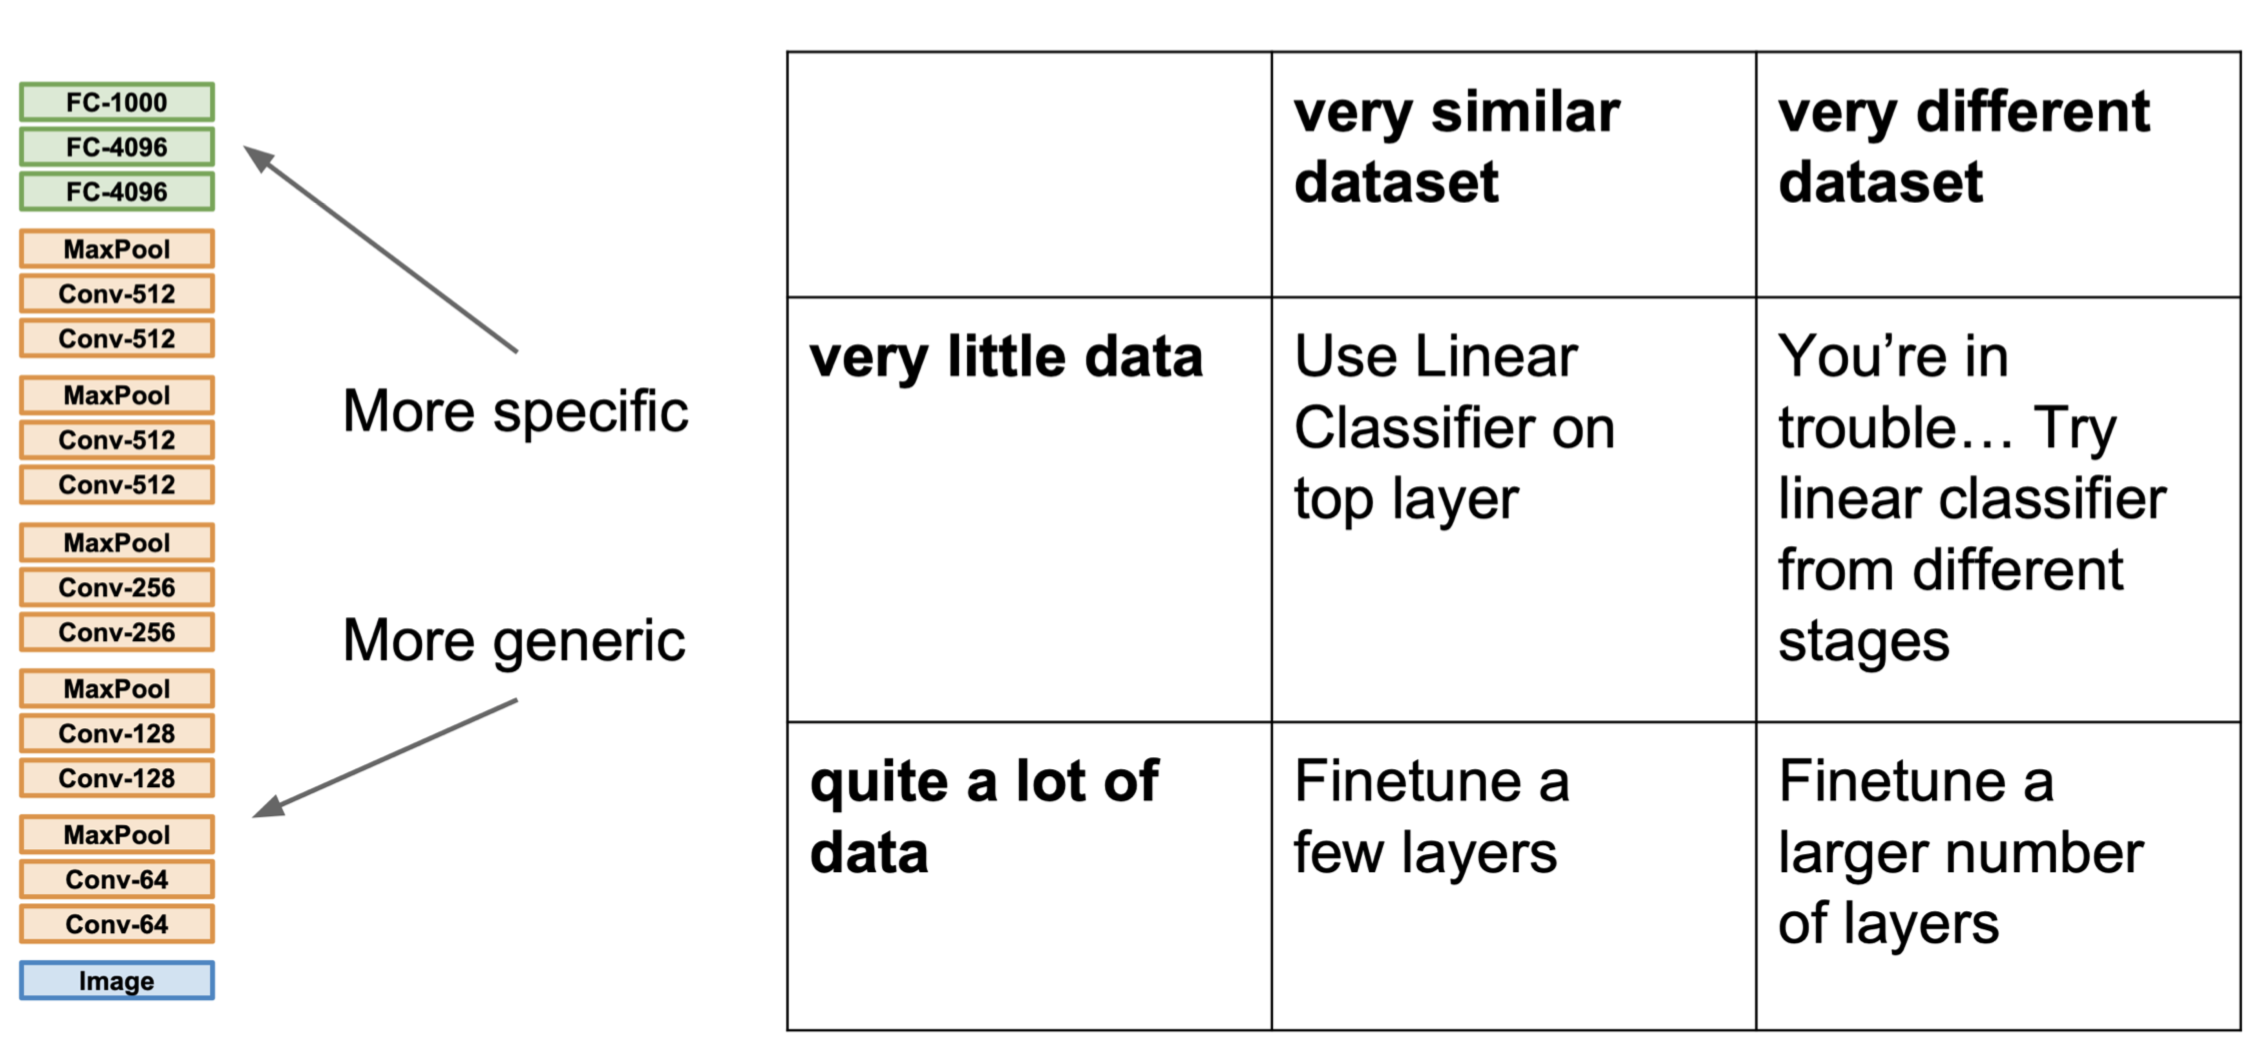
\includegraphics[width=0.5\textwidth]{figures/cv_deep_learning_transfer_learning.png}
	\caption{Transfer learning}
	\label{fig:transfer_learning}
\end{figure}
% cv_deep_learning_transfer_learning.png
\subsection{GANs}
\begin{itemize}
	\item Capture the underlying data distribution and being able to generate new samples
	\item Next to generative adversarial networks, we can also apply Variational Autoencoders or PixelCNN/RNN for this task
	\item GANs are trained by a minimax game between two neural networks (Discriminator $D$ and Generator $G$). $G$ wants to fool $D$ by generating realistic images. $D$ tries to distinguish between generated and real images/data:
	$$\min_G \max_D V(G,D) = \mathbb{E}_{\bm{x}\sim p_{\text{data}}(\bm{x})} \left[\log \left(D\left(\bm{x}\right)\right)\right] + \mathbb{E}_{\bm{z}\sim p_{z}(\bm{z})} \left[\log\left(1 - D\left(G\left(\bm{z}\right)\right)\right)\right] $$
	\item The standard/plain GAN architecture uses a noise vector $\bm{z}$ as input to the generator. Note that it is also possible to put  and condition the GANs input on the output (aka \textit{conditional GANs}). To ensure that the generator learns a relation from input to output, we might need to add an additional loss term like MSE to a label
	\item The training procedure consists of two steps which can be alternated or repeated by themselves for multiple times
	\begin{enumerate}
		\item \textit{Fix $G$ and train $D$}: in order to train the discriminator, we let $G$ generate fake images and feed the discriminator both the fake and sampled real data. Note that we need to fix $G$ to not backpropagate the error of $D$ through $G$.
		\item \textit{Fix $D$ and train $G$}: $G$ is trained by generating images and backpropagating the error of the prediction of $D$ (towards prediction of a real image). Although the gradients flow back through $D$, we do not update any weights of the discriminator as we otherwise cheat (train $D$ to optimize loss of $G$)
	\end{enumerate}
\subsubsection{Stability and Training problems}
	\item In general, it is hard to train a GAN. There are a lot of problems that can occur
	\item \textbf{Vanishing gradients} during training:
	\begin{itemize}
		\item If the discriminator is too bad, the generator does not get valid/accurate feedback and can therefore not learn properly
		\item If the discriminator is perfect, the generator has very low gradients as a small change does not influence the discriminator
		\begin{figure}[ht!]
			\centering
			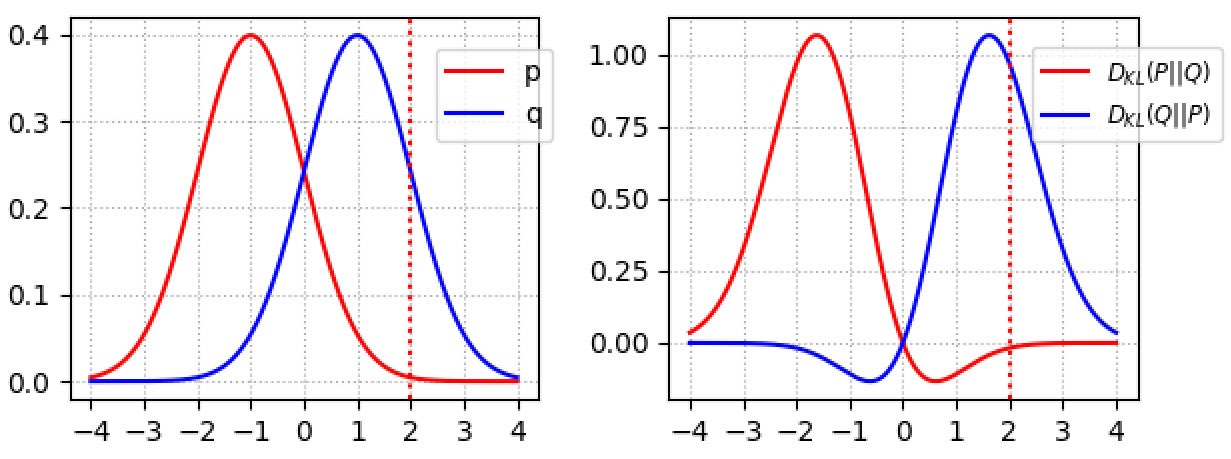
\includegraphics[width=0.4\textwidth]{figures/cv_deep_learning_GAN_vanishing_gradients.jpeg}
			\caption{Vanishing gradients problem for training with KL-divergence. When the distance between the two distributions $p$ and $q$ (respectively $P_g$ and $P_r$) is too huge, the KL divergence is very close to zero. Hence, is does not provide any strong gradients in these regions.}
		\end{figure}
	\end{itemize}
	\item \textbf{Reaching the equilibrium}
	\begin{itemize}
		\item We know that the nash equilibrium of the minimax game is $P_g=P_r$ meaning the distribution of the real data is equal to the generated data. In that case, $D$ return 0.5 no matter what example we put in (as both distributions are equal).
		\item However, it has been shown that such cost functions may not converge when using gradient descent. An example is shown in Figure~\ref{fig:GAN_reaching_equilibrium}.
		\begin{figure}[ht!]
			\centering
			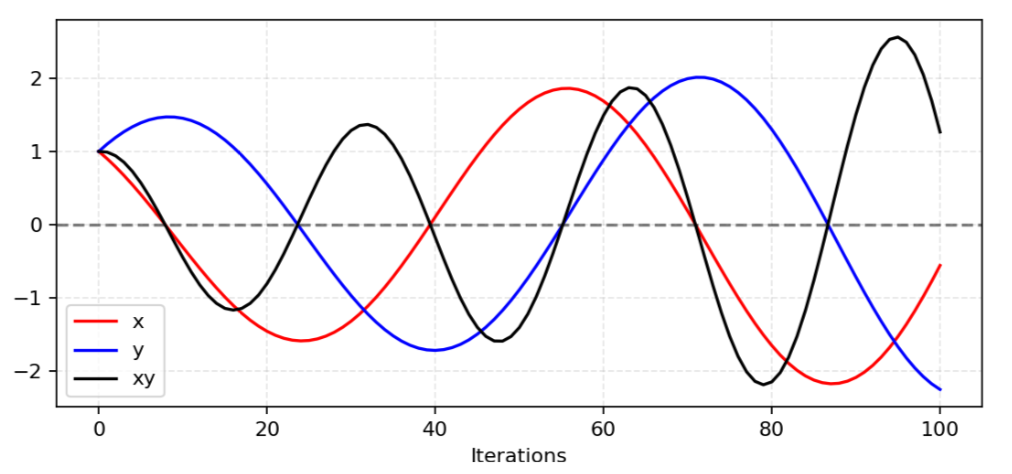
\includegraphics[width=0.4\textwidth]{figures/cv_deep_learning_GAN_oscillating.png}
			\caption{Oscillating behavior of a non-cooperative game where $\min_x \max_y V(x,y) = x\cdot y$. The equilibrium $x=y=0$ is never reached.}
			\label{fig:GAN_reaching_equilibrium}
		\end{figure}
	\end{itemize}
	\item \textbf{Mode collapse}
	\begin{itemize}
		\item A GAN suffers from a mode collapse if the generator limits its predictions/generated distribution to a few samples/modes.
		\item For example in case of the MNIST dataset, this would mean that the generator only creates numbers of one or two different digits. Although a full mode collapse is rarely the case, partial mode collapses frequently occur
		\item In order to create a mode collapse, the gradients regarding the noise $\bm{z}$ must be very low/close to zero. This can for example happen if we fix the discriminator and the generator converges to the optimal image $\bm{x}^*$ that fools the discriminator the most
		\item Once the generator collapse to one mode, the discriminator will learn that this mode is purely/mostly generated and thus changes its predictions. The generator will address that by changing the mode (note that as $\partial L/\partial \bm{z}\approx 0$, we will just collapse to the next mode and are not able to escape this loop).
		\item In the end, this turns into a cat-and-mouse game between the generator and discriminator, and will not converge (see Figure~\ref{fig:GAN_mode_collapse}).
		\begin{figure}[ht!]
			\centering
			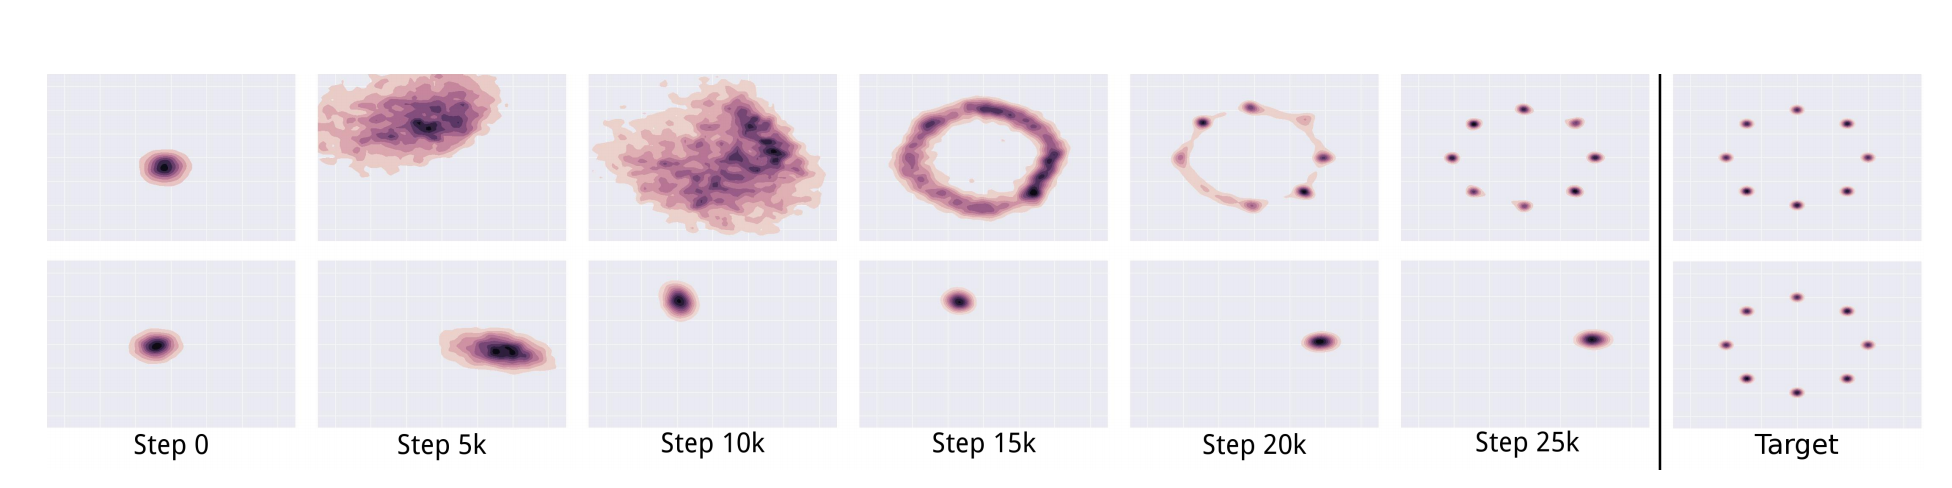
\includegraphics[width=0.6\textwidth]{figures/cv_deep_learning_GAN_mode_collapse.png}
			\caption{\textit{Top row}: optimal convergence of generator distribution to 8 modes. \textit{Bottom row}: Sample of a mode collapse after 10k iterations. The generator is only able to generate a single mode.}
			\label{fig:GAN_mode_collapse}
		\end{figure}
	\end{itemize}
\end{itemize}